\section{Компенсирующий регулятор}
Рассмотрим систему 
\begin{equation}
    \hat{x} = Ax + Bu + B_fw_f, \quad x(0) = \begin{bmatrix}0 & 0 & 0\end{bmatrix}^T
\end{equation}
с генератором внешнего возмущения 
\begin{equation}
    \dot{w}_f = \Gamma w_f, \quad w_f(0) = \begin{bmatrix}1 & 1 & 1 & 1\end{bmatrix}^T
\end{equation}
и виртуальным выходом
\begin{equation}
    z = C_z x 
\end{equation}
где 
\begin{equation}
    \begin{array}{cc}
        \begin{array}{ccc}
            A = \begin{bmatrix}
                8 & 1 & 11 \\ 
                4 & 0 & 4 \\ 
                -4 & -3 & -7 \\ 
            \end{bmatrix}, & 
            B = \begin{bmatrix} -1 \\ -3 \\ 3 \end{bmatrix}, &
            B_f = \begin{bmatrix}
                0 & 1 & -1 & 0 \\ 
                0 & 0 & 0 & 0 \\
                0 & -1 & 0 & 0 \\
            \end{bmatrix}, 
        \end{array} \\ 
        \begin{array}{cc}
        C_z = \begin{bmatrix} -2 \\ -3 \\ -1 \end{bmatrix}^T, & 
        \Gamma = \begin{bmatrix}
            -40 & 16 & 9 & 7 \\ 
            -64 & 25 & 14 & 12 \\
            -26 & 11 & 7 & 3 \\ 
            -48 & 18 & 14 & 8 \\ 
        \end{bmatrix}
        \end{array}
    \end{array}
\end{equation}

Схема моделирования этой системы приведена на рисунке \ref{fig:scheme1}.
\begin{figure}[ht!]
    \centering
    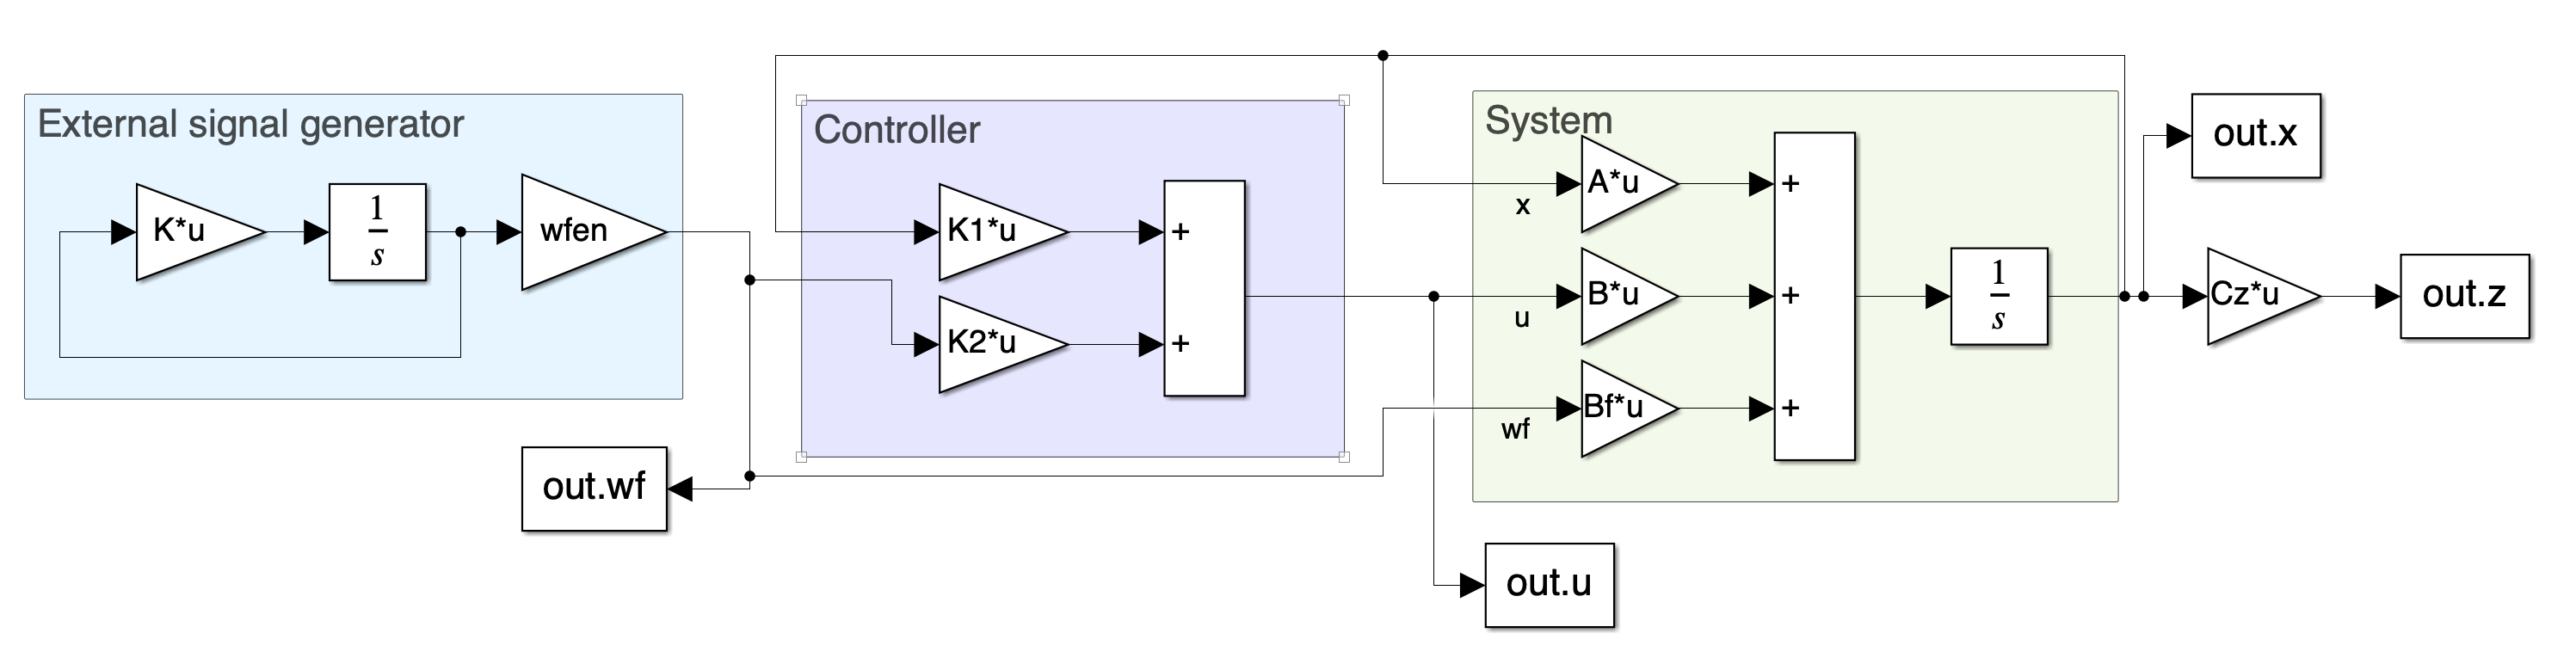
\includegraphics[width=\textwidth]{media/scheme1.png}
    \caption{Схема моделирования системы}
    \label{fig:scheme1}
\end{figure}

\subsection{Анализ внешнего возмущения}
Так как внешние возмущение задается линейной системой, можно найти его собственные числа, из которых 
будет понятен общий вид его выражения. 
\begin{equation}
    \sigma(\Gamma) =  \begin{bmatrix}
        0 \pm 3j & 
        0 \pm 2j 
    \end{bmatrix}
\end{equation}
Таким образом, так как вещественная часть всех собственных чисел 
матрицы равны нули, в комплексные части являются попарно сопряженными, 
то можно сказать, что внешнее возмущение будет иметь гармонический характер, 
состоящий из двух частотных составляющих. 

Можно найти уравнение внешнего возмущения: 
\begin{equation}
    w_f = e^{\Gamma t} \cdot w_f(0) 
\end{equation}
График внешнего возмущения приведен на рисунке \ref{fig:wf}.
\begin{figure}[ht!]
    \centering
    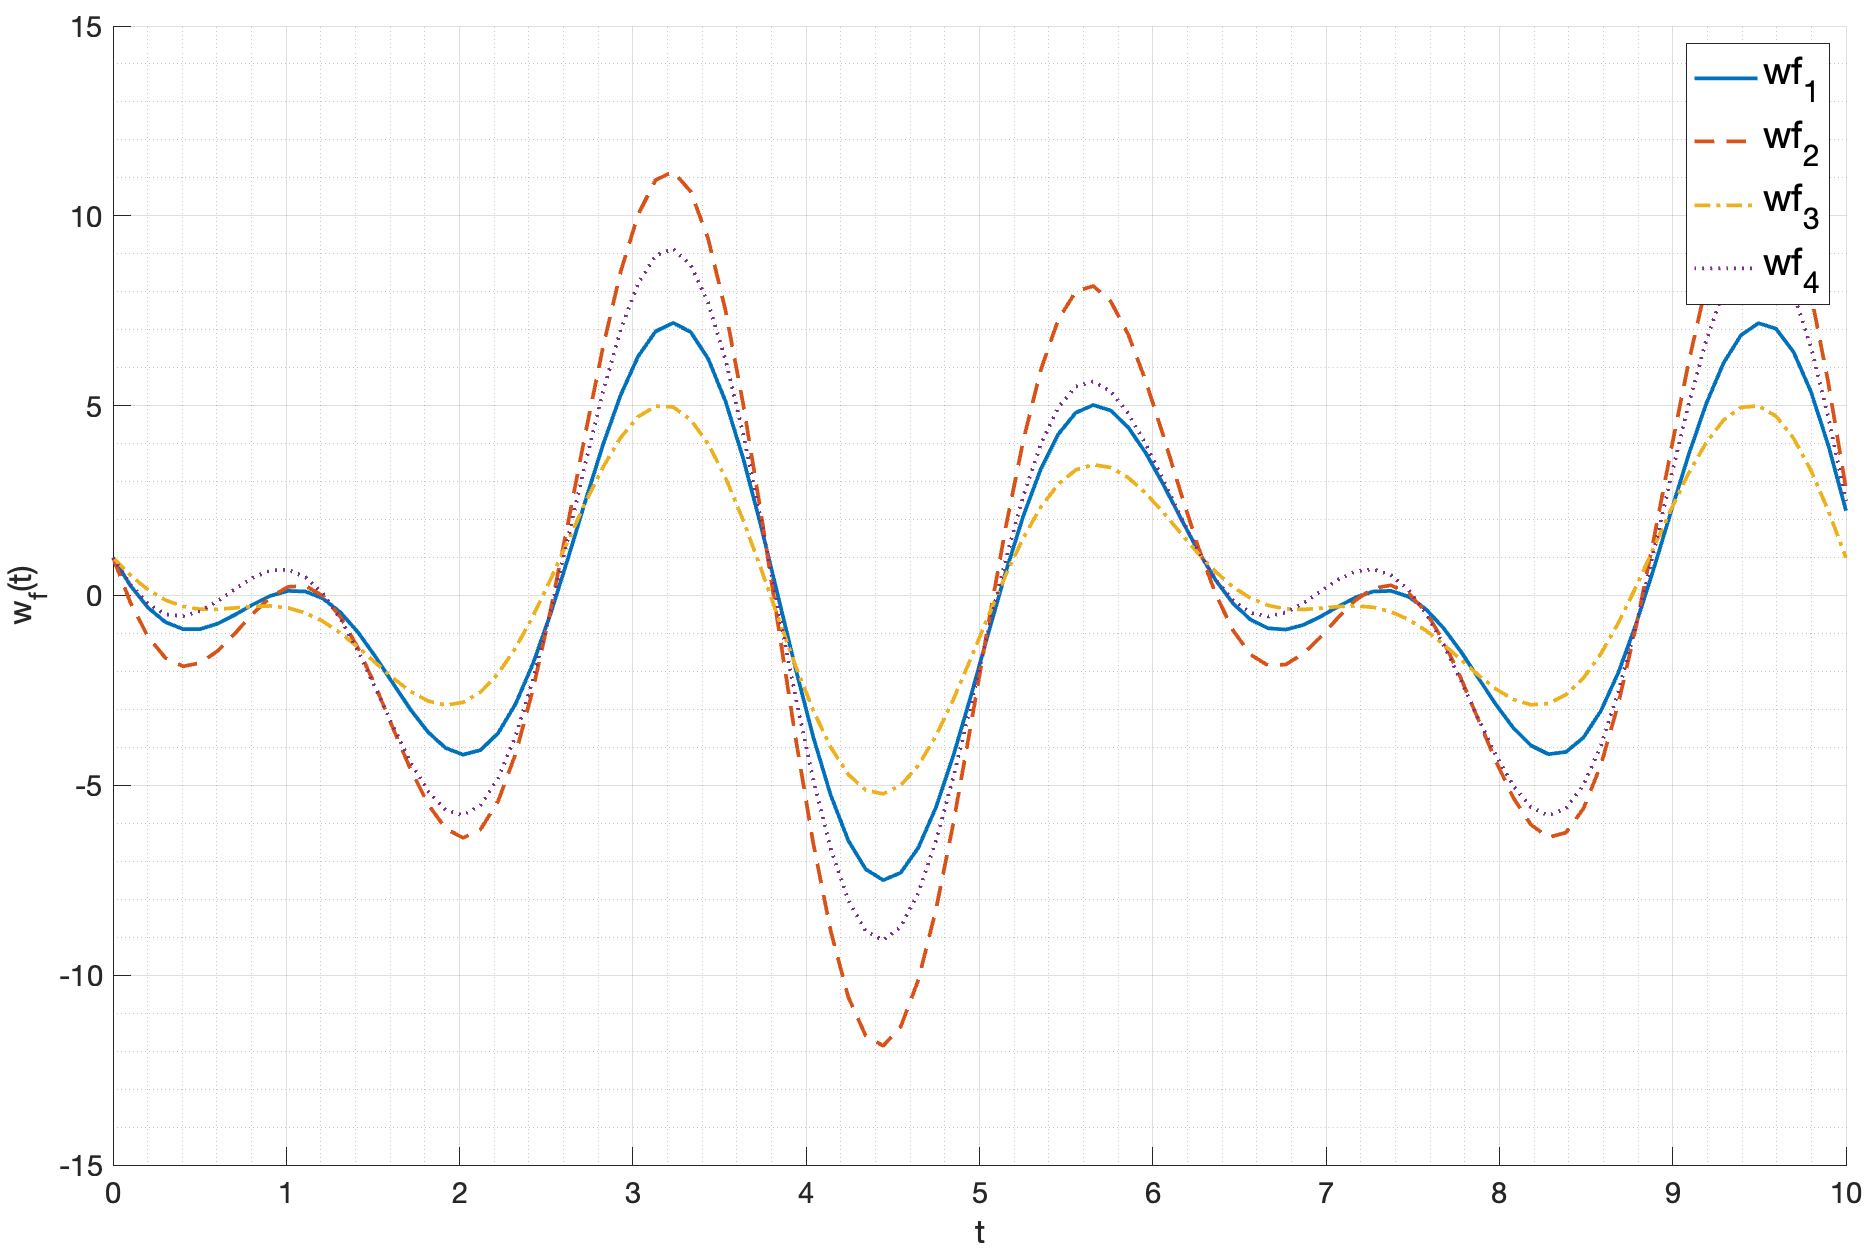
\includegraphics[width=\textwidth]{media/plots/wf.png}
    \caption{График внешнего возмущения}
    \label{fig:wf}
\end{figure} 
Реакция разомкнутой системы ($u = 0$) при начальных условиях $x(0) = \begin{bmatrix}0 & 0 & 0 \end{bmatrix}^T$ 
на внешнее возмущение приведена на рисунках \ref{fig:open_x}, \ref{fig:open_z} (состояние системы и виртуальный выход соответственно).
\begin{figure}[ht!]
    \centering
    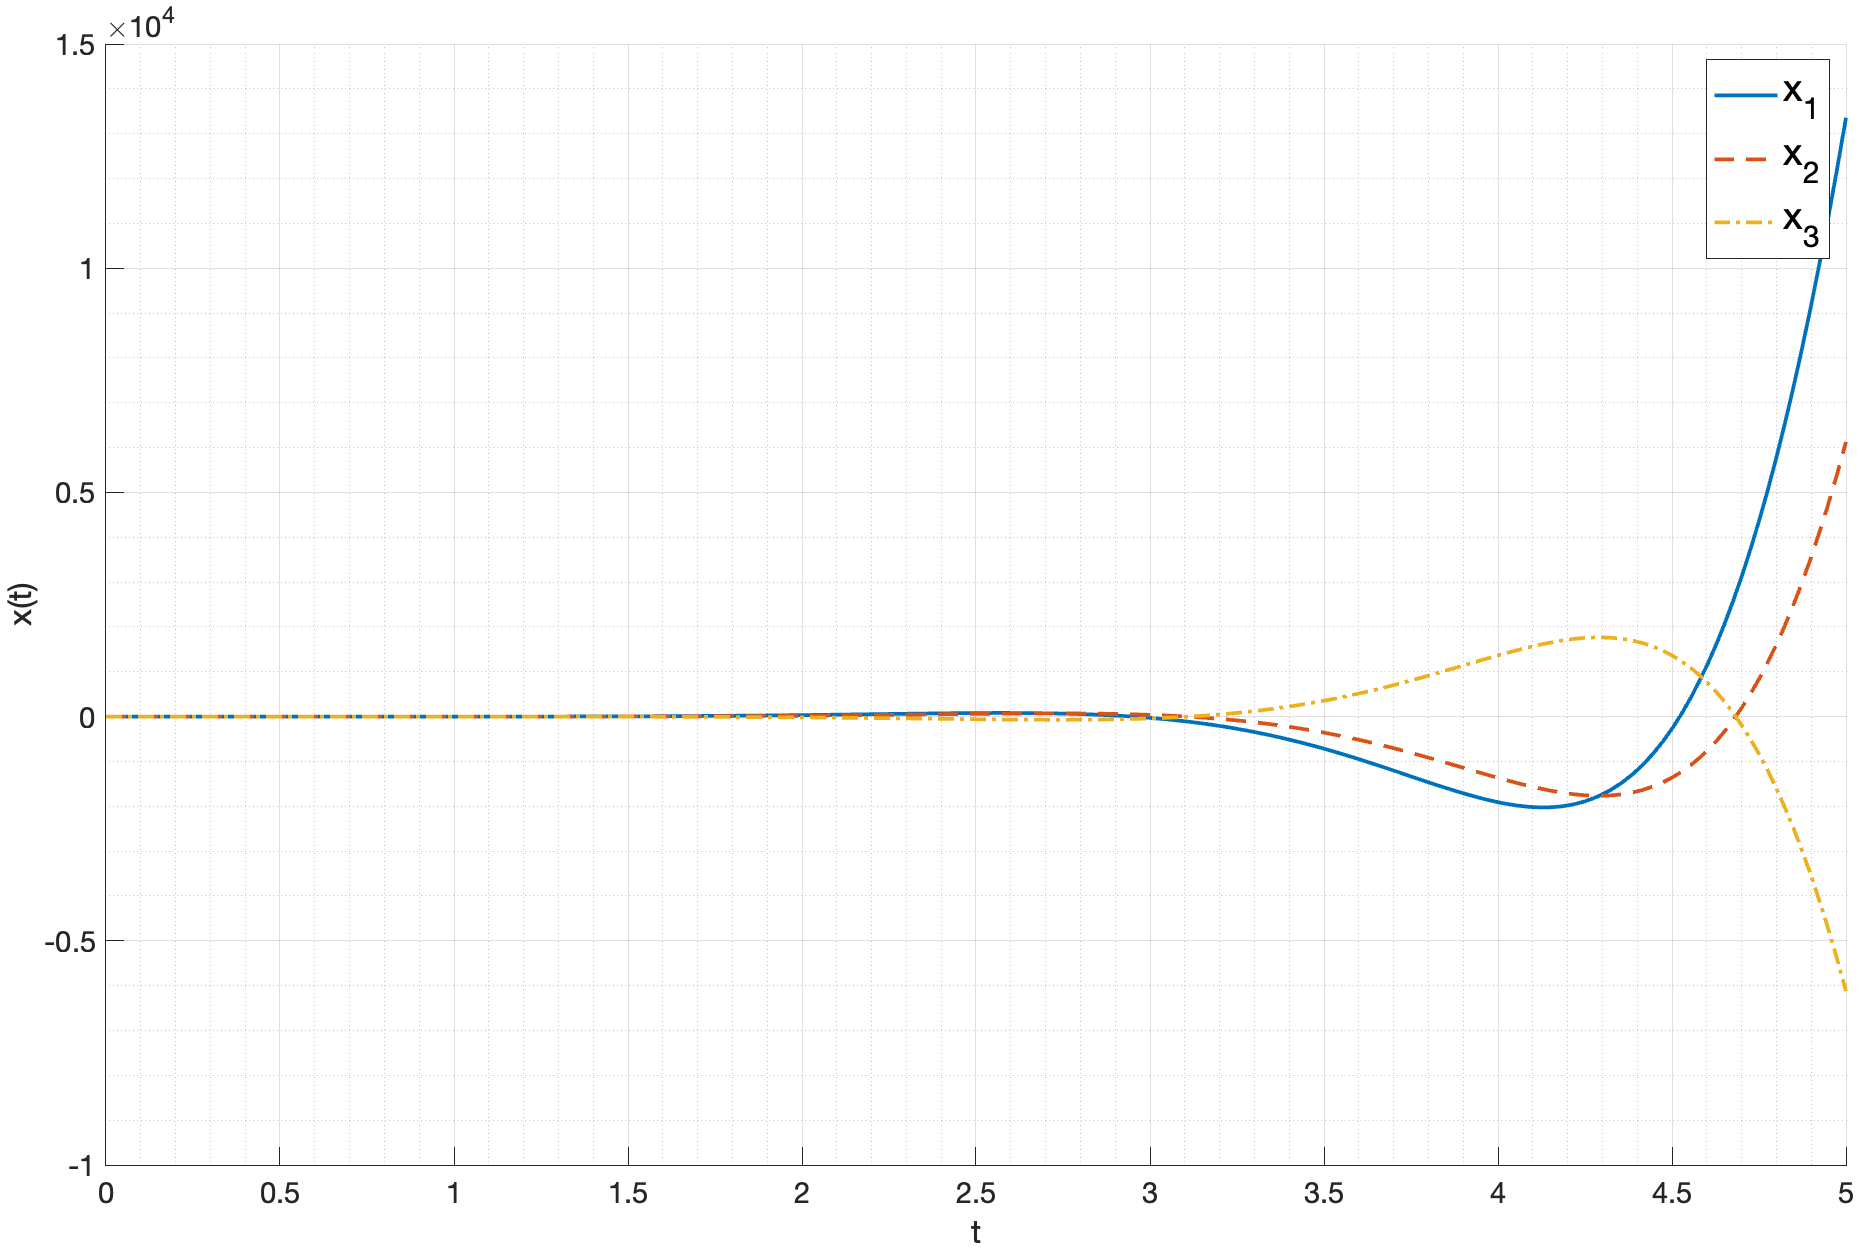
\includegraphics[width=\textwidth]{media/plots/open_x.png}
    \caption{Реакция разомкнутой системы на внешнее возмущение (состояние системы)}
    \label{fig:open_x}
\end{figure}
\begin{figure}[ht!]
    \centering
    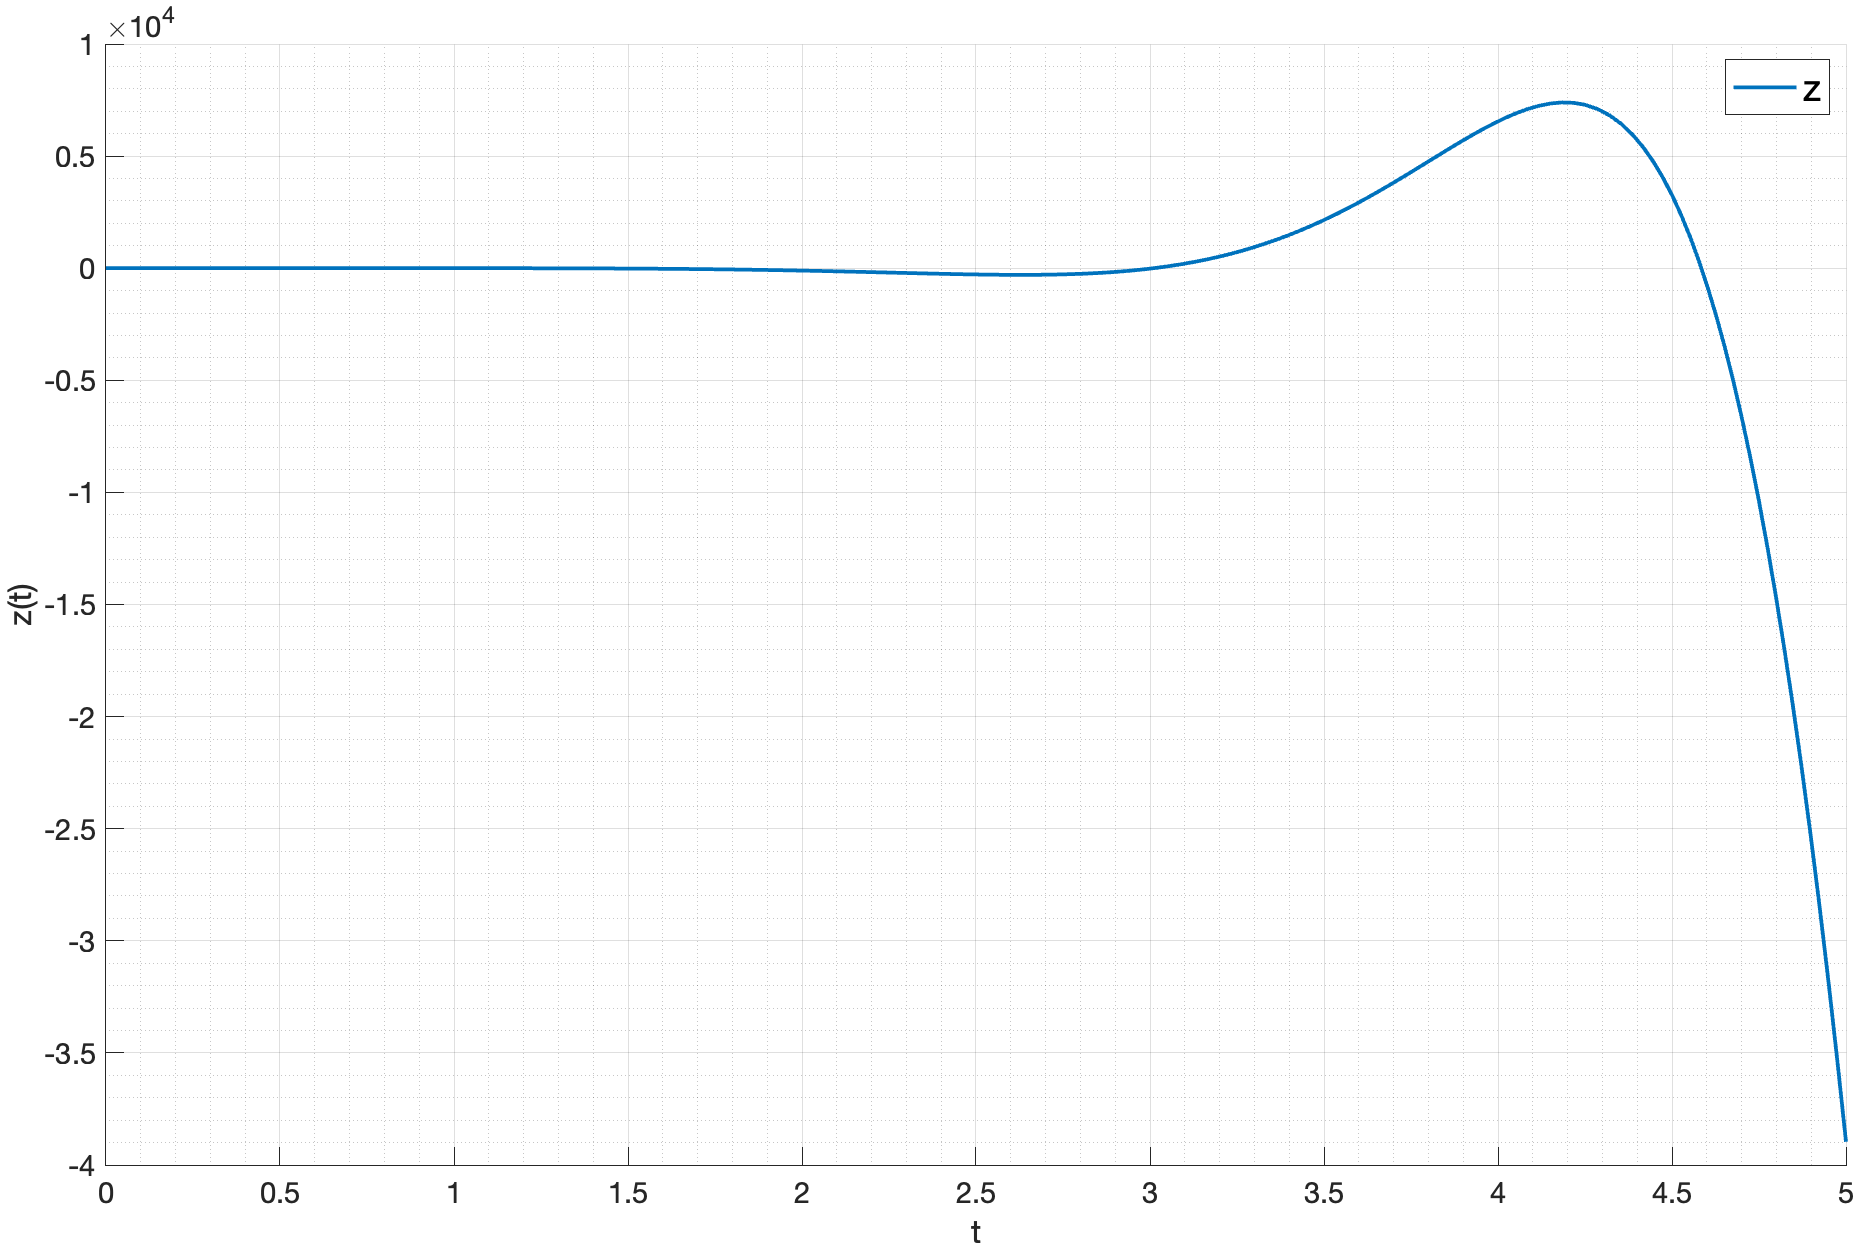
\includegraphics[width=\textwidth]{media/plots/open_z.png}
    \caption{Реакция разомкнутой системы на внешнее возмущение (виртуальный выход)}
    \label{fig:open_z}
\end{figure}
Как видно на графиках, система не является устойчивой. Это связано и с тем, что
собственные числа матрицы $A$ имеют положительную вещественную часть, и с тем, что
внешнее возмущение имеет гармонический характер.

\FloatBarrier
\subsection{Синтез регулятора}
Синтез регулятора, способного компенсировать внешнее возмущение, будет состоять из двух частей. 
Первая -- синтез feedback компоненты, которая обеспечит стабилизацию системы. Для его синтеза
можно воспользоваться модальными или немодальными методами. Вторая -- синтез feedforward компоненты,
которая обеспечит компенсацию внешнего возмущения.

\subsubsection{Управляемость системы}
Перед тем, как приступить к синтезу регулятора, проверим управляемость собственных 
чисел системы. Для этого найдем диагональную форму системы без внешнего возмущения.
\begin{eqnarray}
    A_j = \begin{bmatrix}
        -3.00  & 0.00  & 0.00 \\ 
        0.00  & 2.00  & -2.00 \\ 
        0.00  & 2.00  & 2.00 \\ 
    \end{bmatrix} &
    B_j = \begin{bmatrix}
    -0.00 \\ 
    2.12 \\ 
    4.95 \\ 
    \end{bmatrix}
\end{eqnarray}

собственное число $\lambda_1 = -3$ не является управляемым, но является стабилизируемым. 
Собственные числа $\lambda_2 = 2 \pm 2j$ являются управляемыми. 

\subsubsection{Feedback компонента}
Для синтезе регулятора вида $u = K_1x$ воспользуемся методом немодального синтеза решением матричного неравенства Ляпунова с 
минимизацией нормы управления. Подробно синтез такого регулятора был рассмотрен в прошлой работе. 
\begin{equation}
    \begin{array}{cc}
        PA^T + AP + 2\alpha P + Y^T B^T + BY \preceq 0, ~~~ H = Y P^{-1}, ~~~ P \succ 0 \\ 
        \begin{bmatrix}
            P & x(0) \\
            x(0)^T & 1
        \end{bmatrix} \succ 0, ~~~ \begin{bmatrix}
            P & Y^T \\ 
            Y & \mu^2I
        \end{bmatrix} \succ 0
    \end{array}
\end{equation} 
где $\mu$ -- ограничение на управление $\mu \ge \|u(t)\|_2$.
Минимизируя $\mu$ при заданной степени устойчивости $\alpha = 3$ и начальном 
состоянии $x(0) = \begin{bmatrix}0 & 0 & 0 & 0\end{bmatrix}^T$, получаем следующий регулятор: 
\begin{equation}
    K_1 = \begin{bmatrix}
        -4.57  & 0.29  & -4.57 \\ 
    \end{bmatrix}
    \label{eq:K1}
\end{equation}
Собственные числа системы, замкнутой регулятором $K_1$:
\begin{equation}
    \sigma(A + BK_1) = \begin{bmatrix}
        -3.00 + 4.55j \\ 
        -3.00 - 4.55j \\ 
        -3.00 \\ 
    \end{bmatrix}
\end{equation}
Можно сделать вывод, что регулятор $K_1$ синтезирован корректно. 
Проведем промежуточные исследования системы. Промоделируем систему с регулятором $K_1$ 
без внешнего возмущения и с ним. 
В качестве начальных условий возьмем $x(0) = \begin{bmatrix}1 & 1 & 1\end{bmatrix}^T$.
График состояния системы без внешнего возмущения приведен на рисунке \ref{fig:K1_free_x} 
(состояние системы) и \ref{fig:K1_free_z} (виртуальный выход),
а с внешним возмущением на рисунке \ref{fig:K1_wf_x} (состояние системы) и \ref{fig:K1_wf_z} (виртуальный выход).
\begin{figure}[ht!]
    \centering
    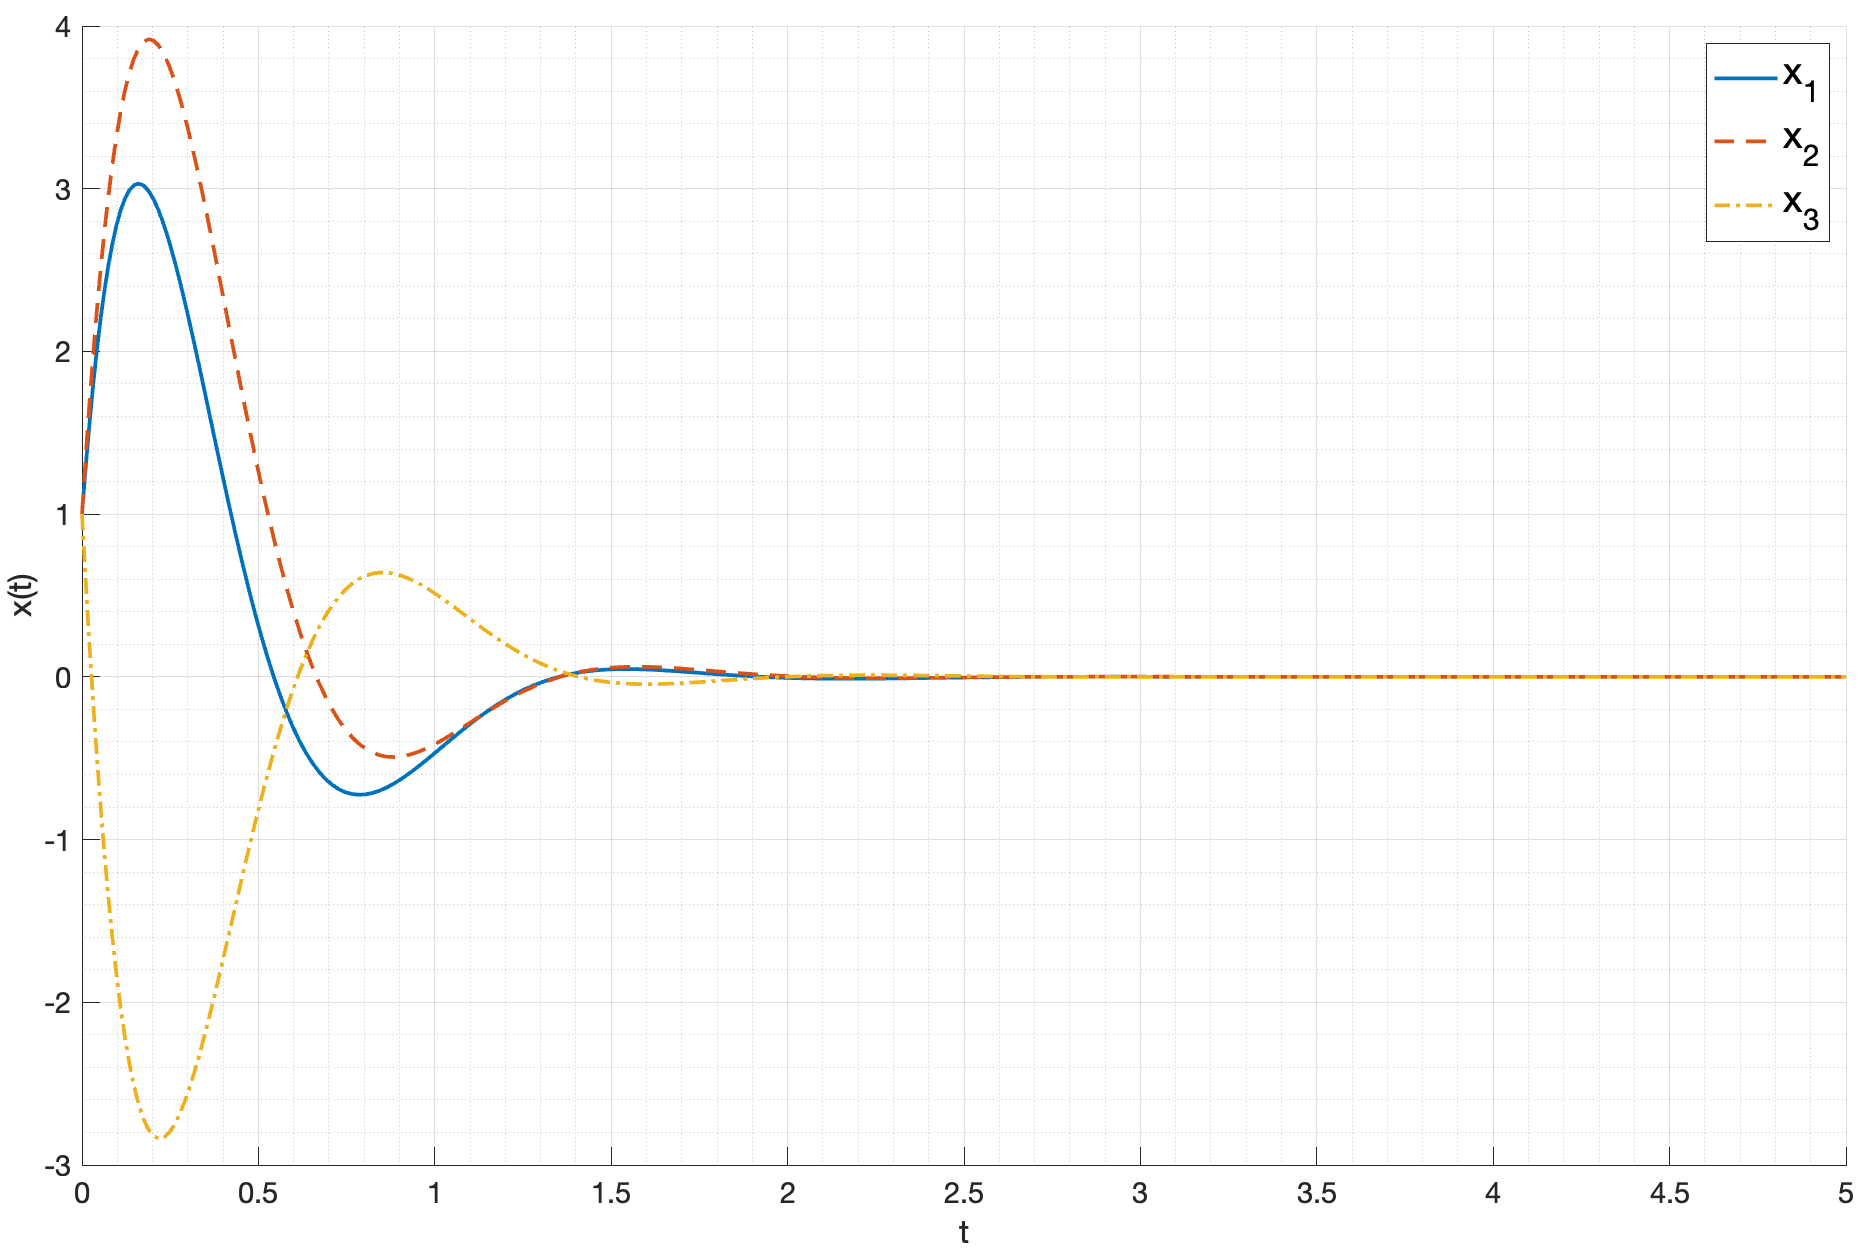
\includegraphics[width=\textwidth]{media/plots/K1_free_x.png}
    \caption{Состояние системы с регулятором $K_1$ без внешнего возмущения}
    \label{fig:K1_free_x}
\end{figure}
\begin{figure}[ht!]
    \centering
    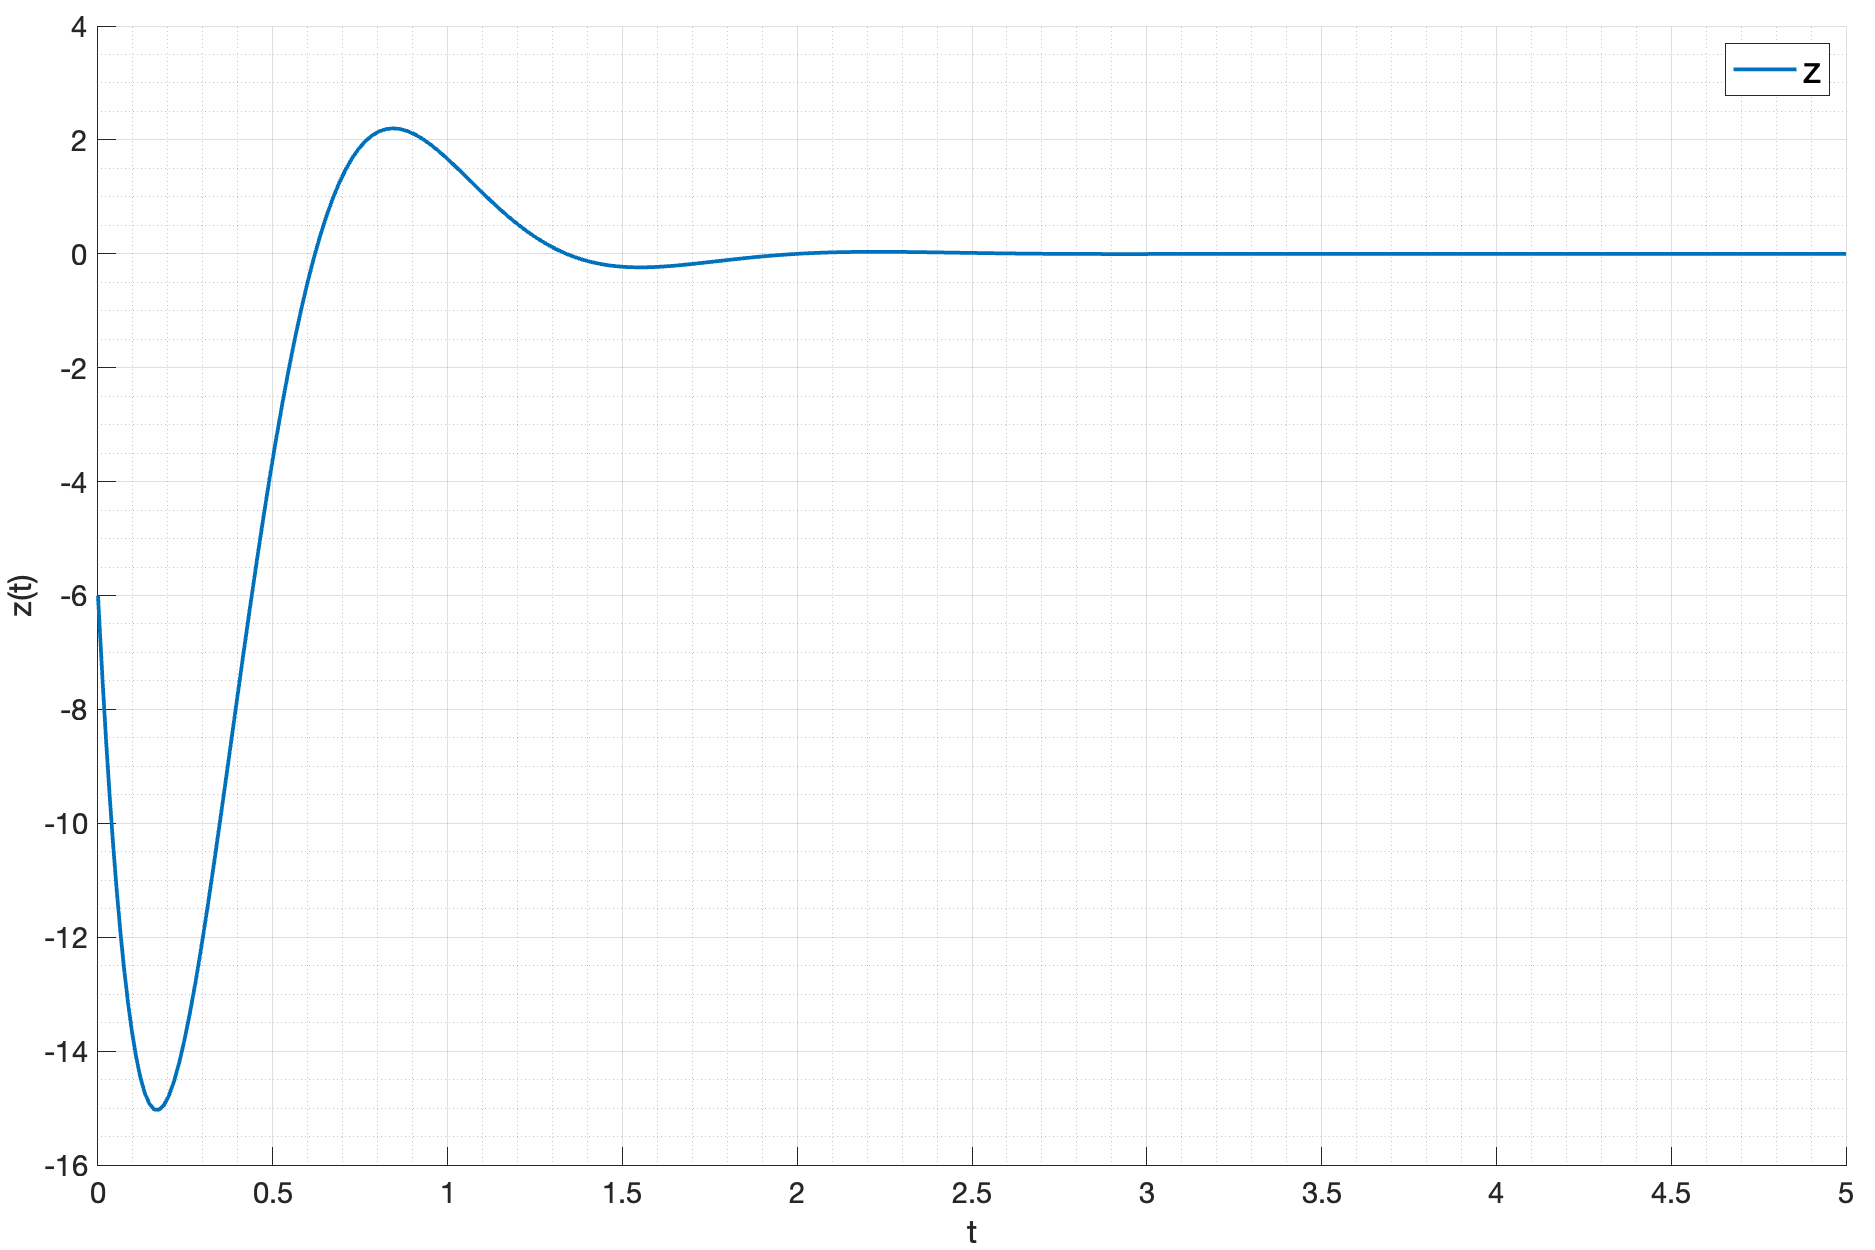
\includegraphics[width=\textwidth]{media/plots/K1_free_z.png}
    \caption{Выход системы с регулятором $K_1$ без внешнего возмущения}
    \label{fig:K1_free_z}
\end{figure}
\begin{figure}[ht!]
    \centering
    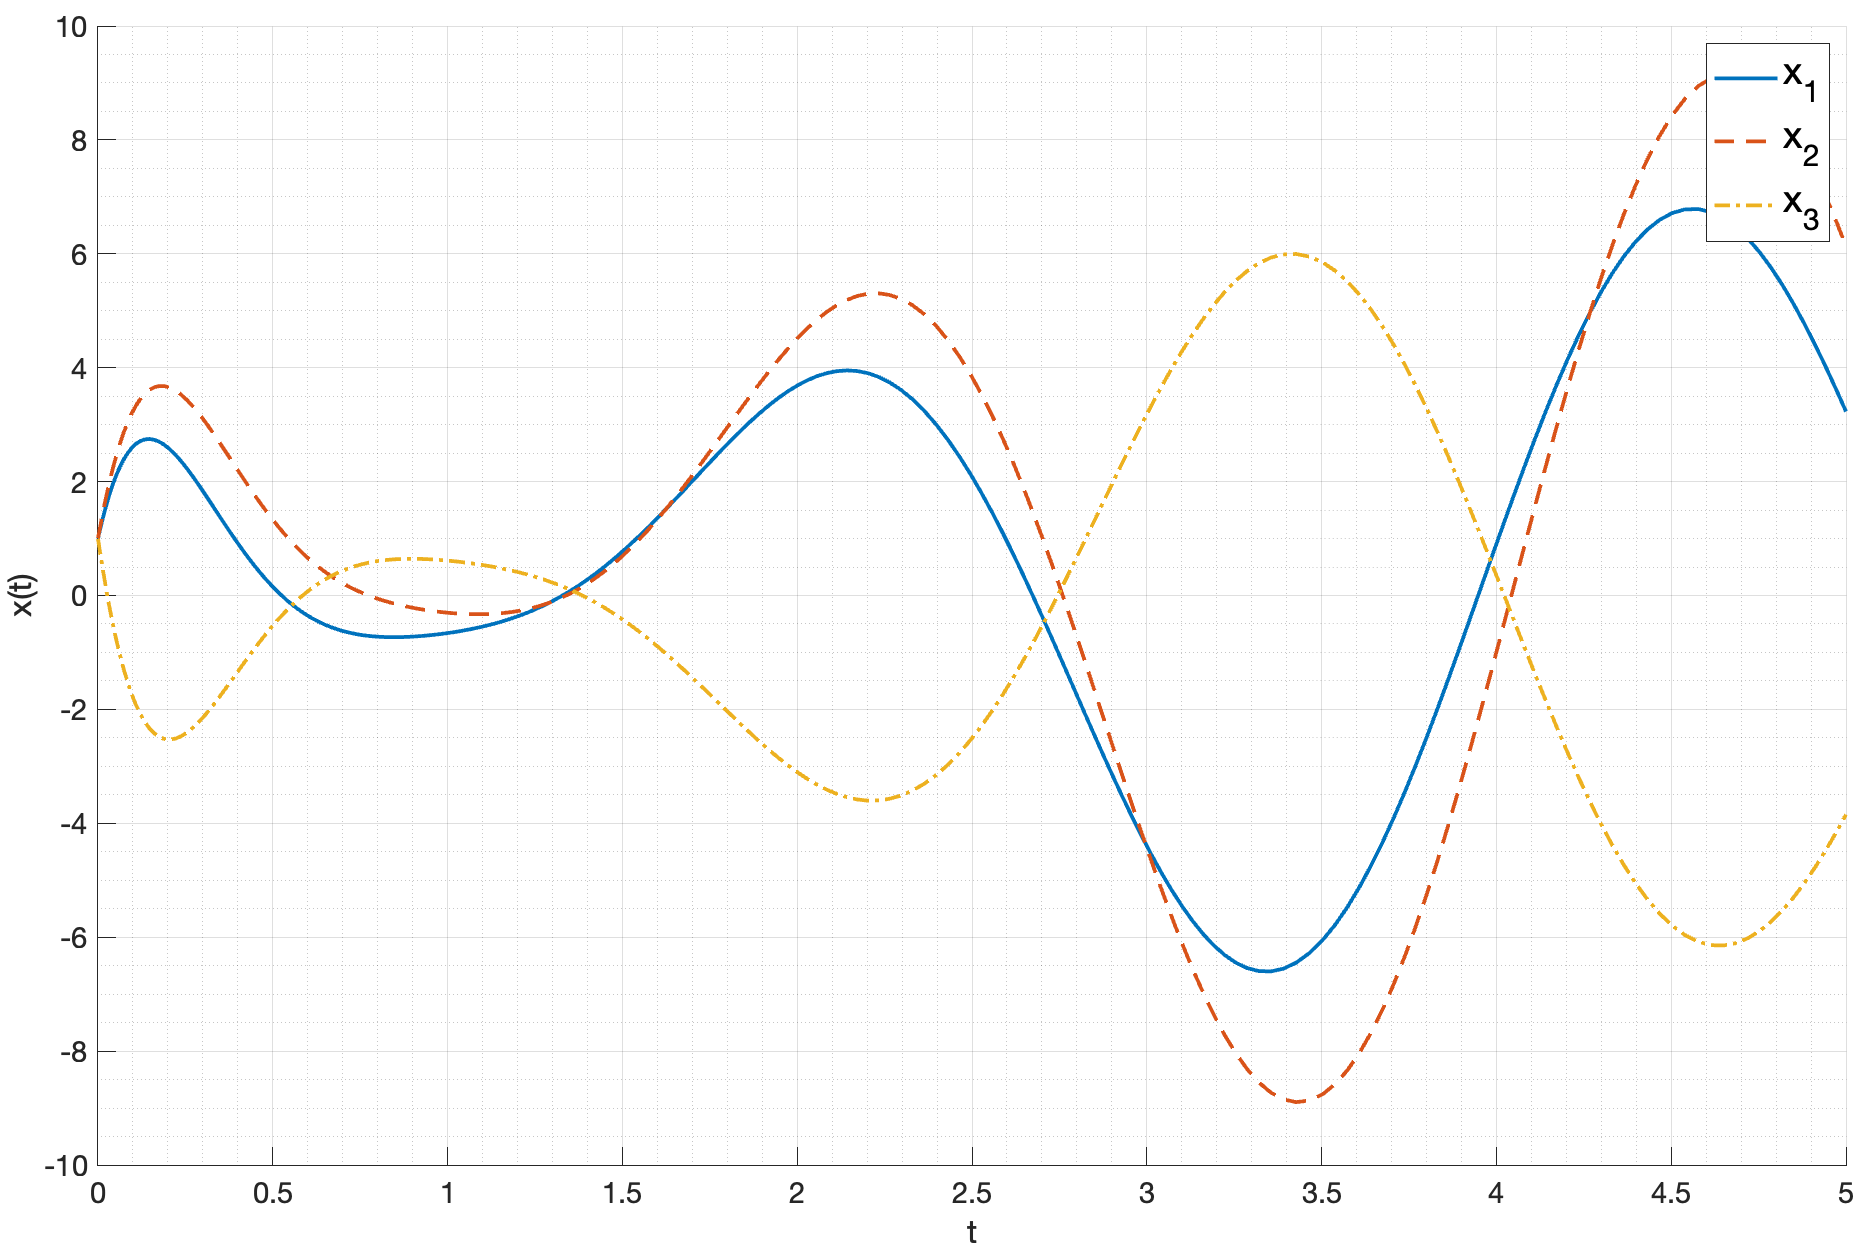
\includegraphics[width=\textwidth]{media/plots/K1_wf_x.png}
    \caption{Состояние системы с регулятором $K_1$ с внешним возмущением}
    \label{fig:K1_wf_x}
\end{figure}
\begin{figure}[ht!]
    \centering
    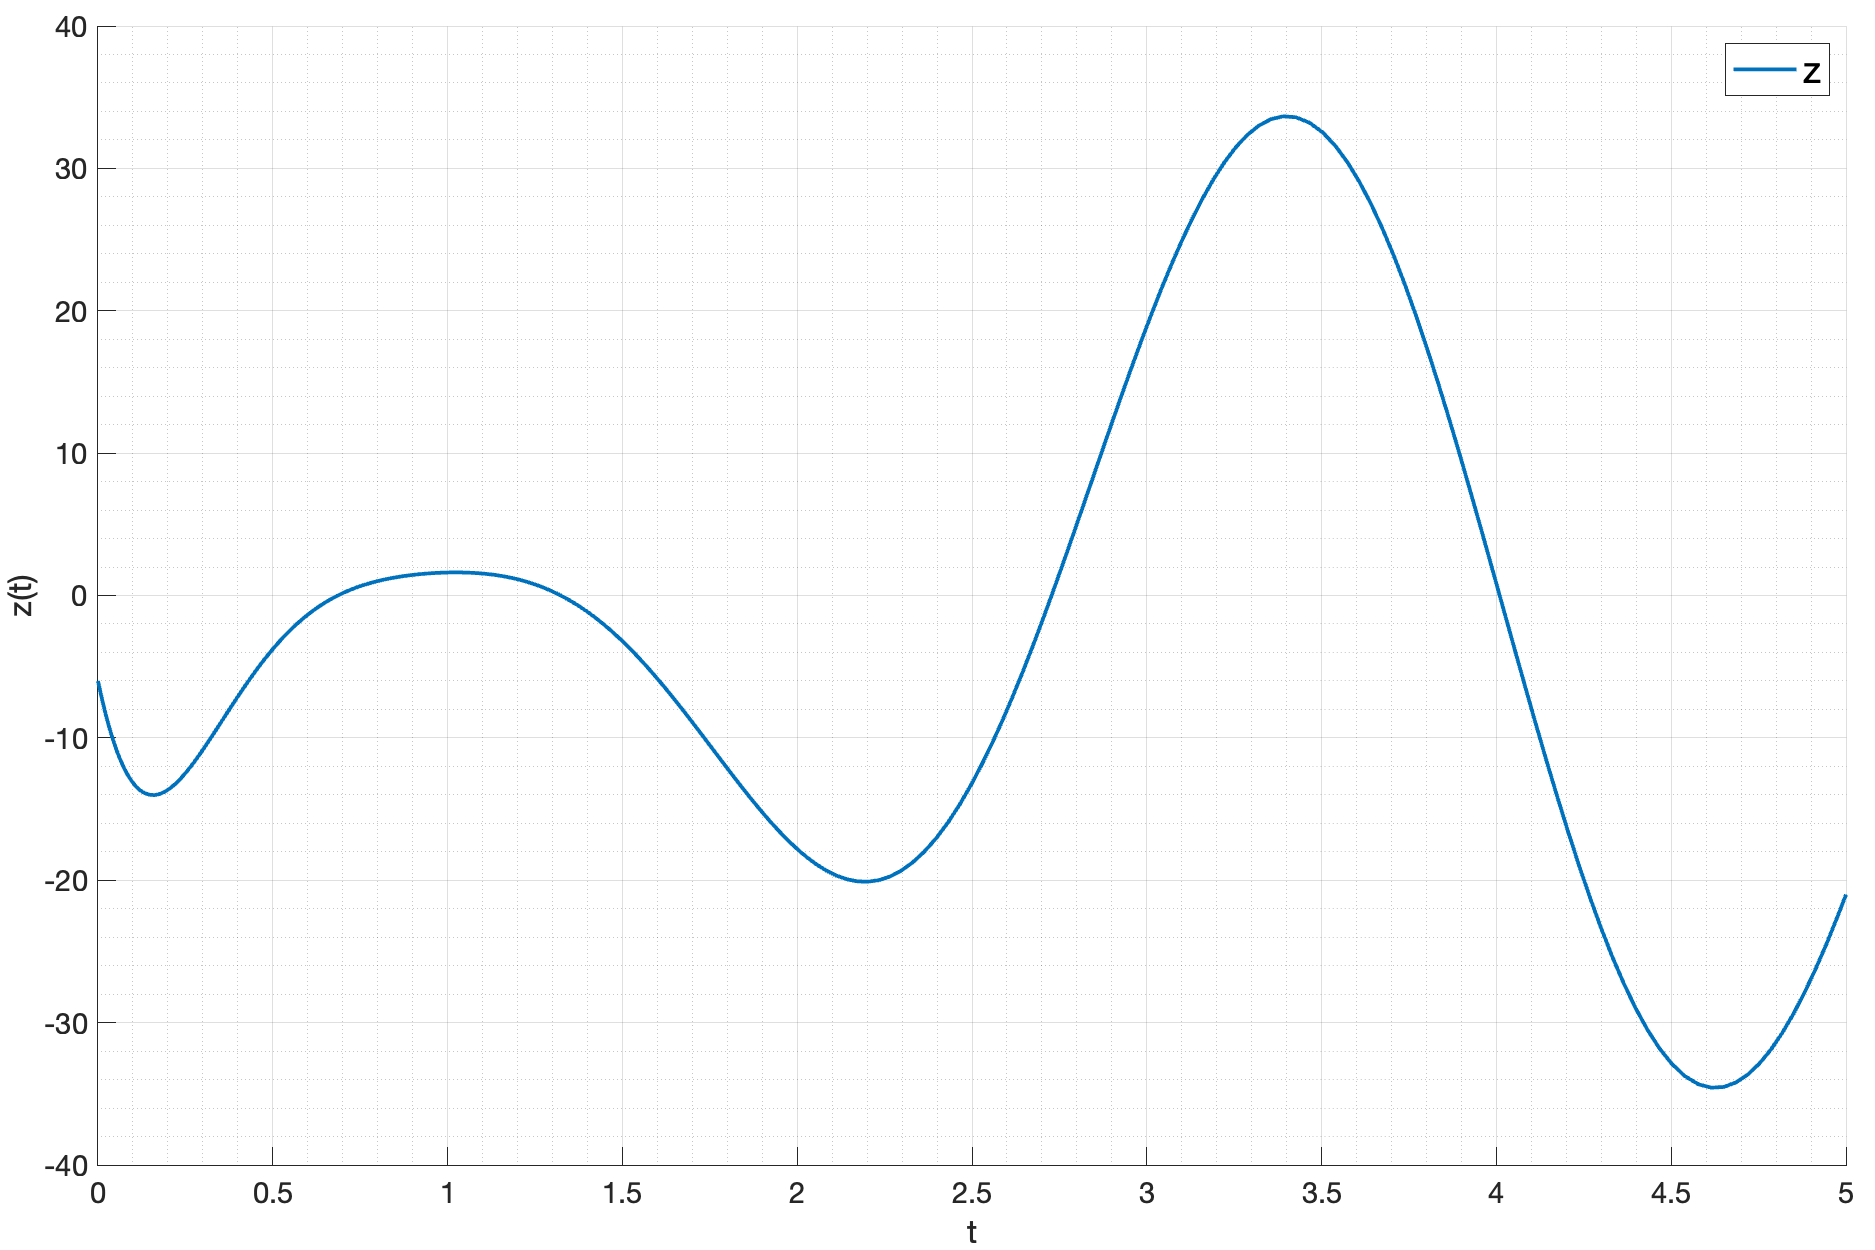
\includegraphics[width=\textwidth]{media/plots/K1_wf_z.png}
    \caption{Выход системы с регулятором $K_1$ с внешним возмущением}
    \label{fig:K1_wf_z}
\end{figure}
\FloatBarrier
Видно, что система, замкнутая регулятором $K_1$ без внешнего воздействия сходится к нулю, 
что подтверждает корректность синтеза регулятора. Но при этом система с внешним возмущением
не имеет устойчивого состояния.
\FloatBarrier
\subsubsection{Feedforward компонента}
Для синтеза компенсирующего регулятора воспользуемся уравнениями: 
\begin{equation}
    \begin{cases}
        P\Gamma - AP = BY + B_f \\ 
        C_z P = 0 \\ 
        K_2 = Y - K_1 P \\ 
    \end{cases}
\end{equation}
Условием существования такого регулятора является принадлежность собственных чисел 
внешнего возмущения правой комплексной полуплоскости и принадлежность корней 
системы, замкнутой регулятором, левой комплексной полуплоскости. Оба эти условия выполняются. 
Решим систему с помощью пакета \texttt{cvx} в MATLAB, в результате получаем:
\begin{equation}
    K_2 = \begin{bmatrix}
        -5.96  & 2.25  & 2.72  & 1.48 \\ 
    \end{bmatrix} 
\end{equation}

Проверим синтезированный регулятор на устойчивость при внешнем возмущении. 
График моделирования системы с внешним воздействием и начальными условиями 
$x(0) = \begin{bmatrix}0 & 0 & 0\end{bmatrix}^T$ с использованием \textit{полного}
регулятора $u = K_1x + K_2w_f$ приведен на рисунках \ref{fig:K_full_x} (состояние системы) и \ref{fig:K_full_z} (виртуальный выход).
\begin{figure}[ht!]
    \centering
    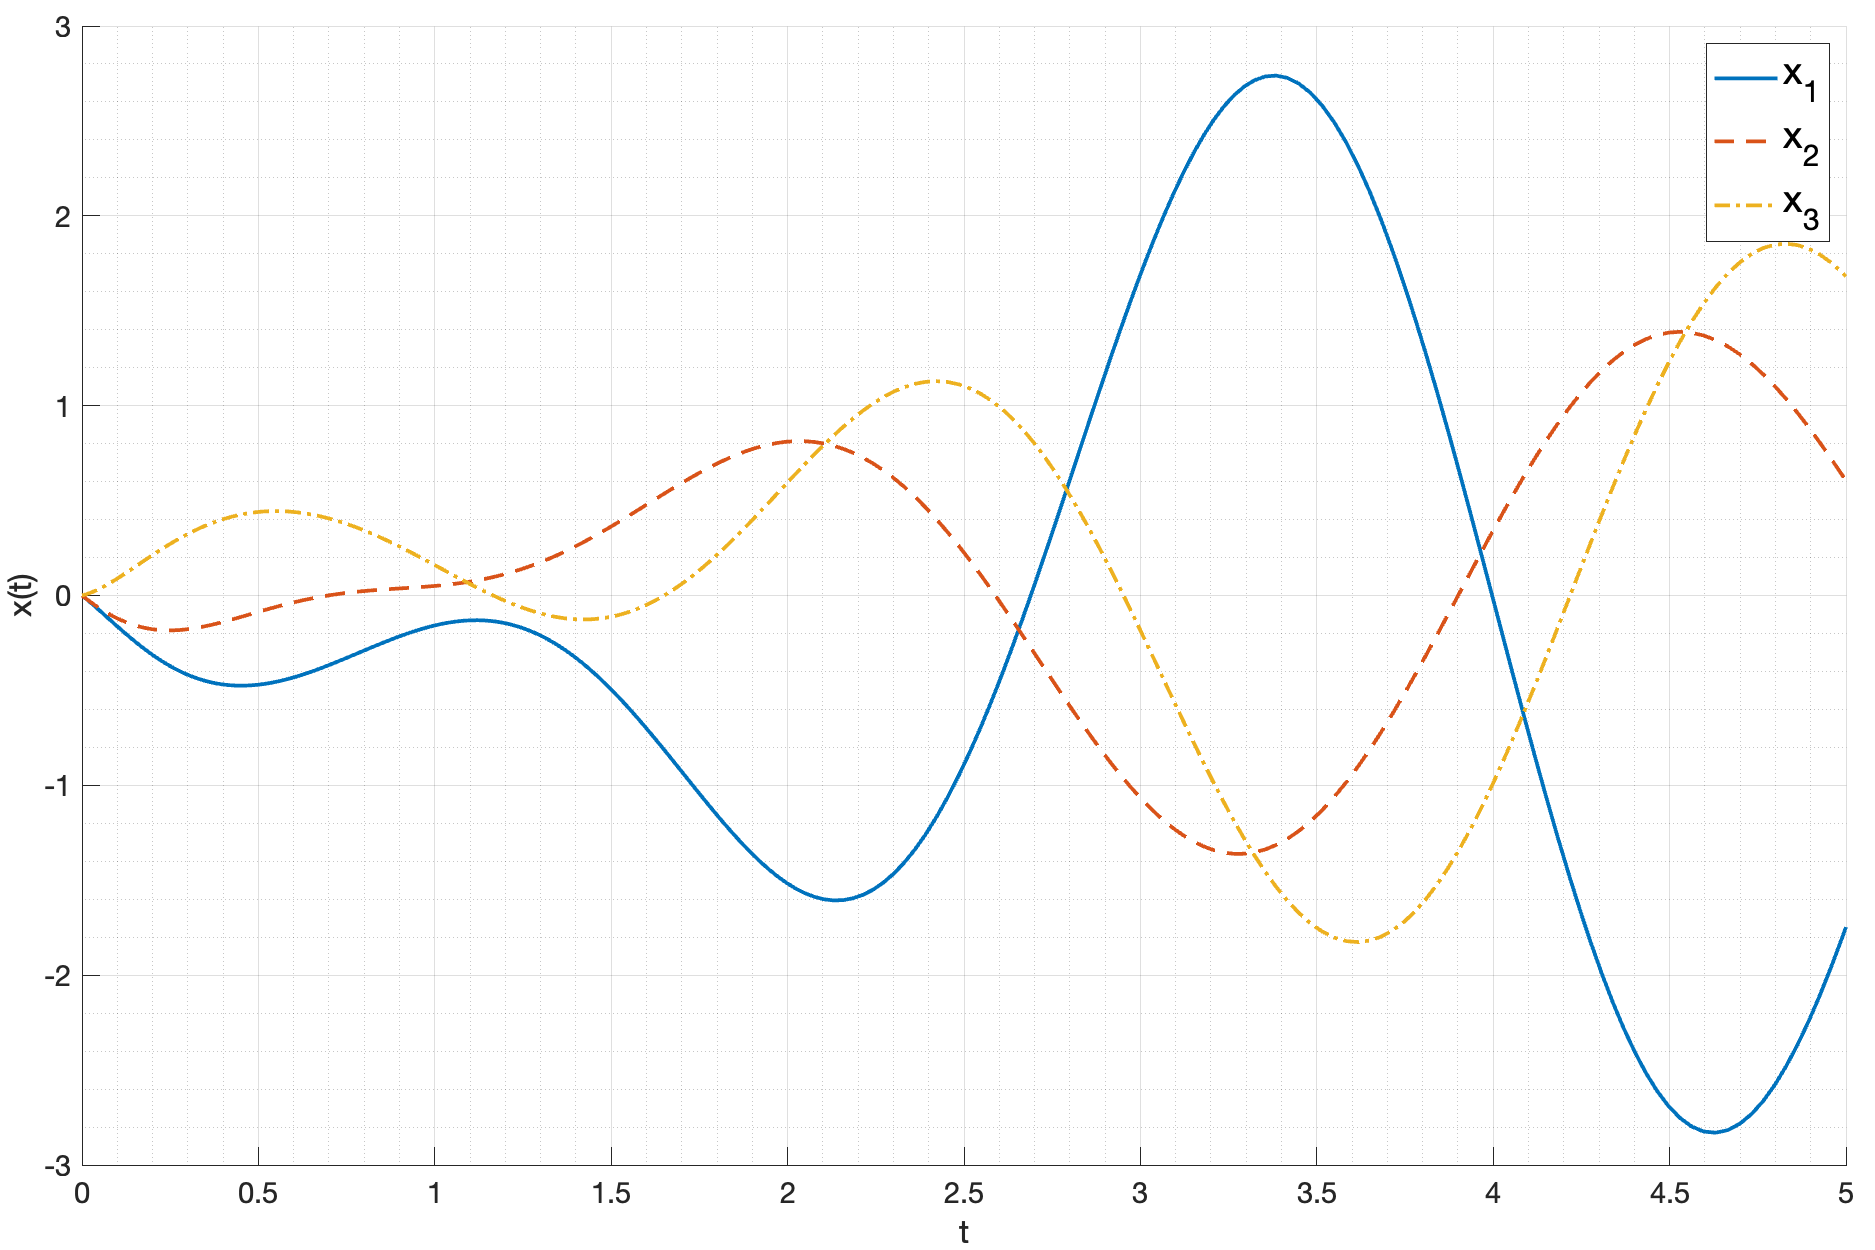
\includegraphics[width=\textwidth]{media/plots/full_x.png}
    \caption{Состояние системы с полным регулятором $K_1 + K_2$}
    \label{fig:K_full_x}
\end{figure}
\begin{figure}[ht!]
    \centering
    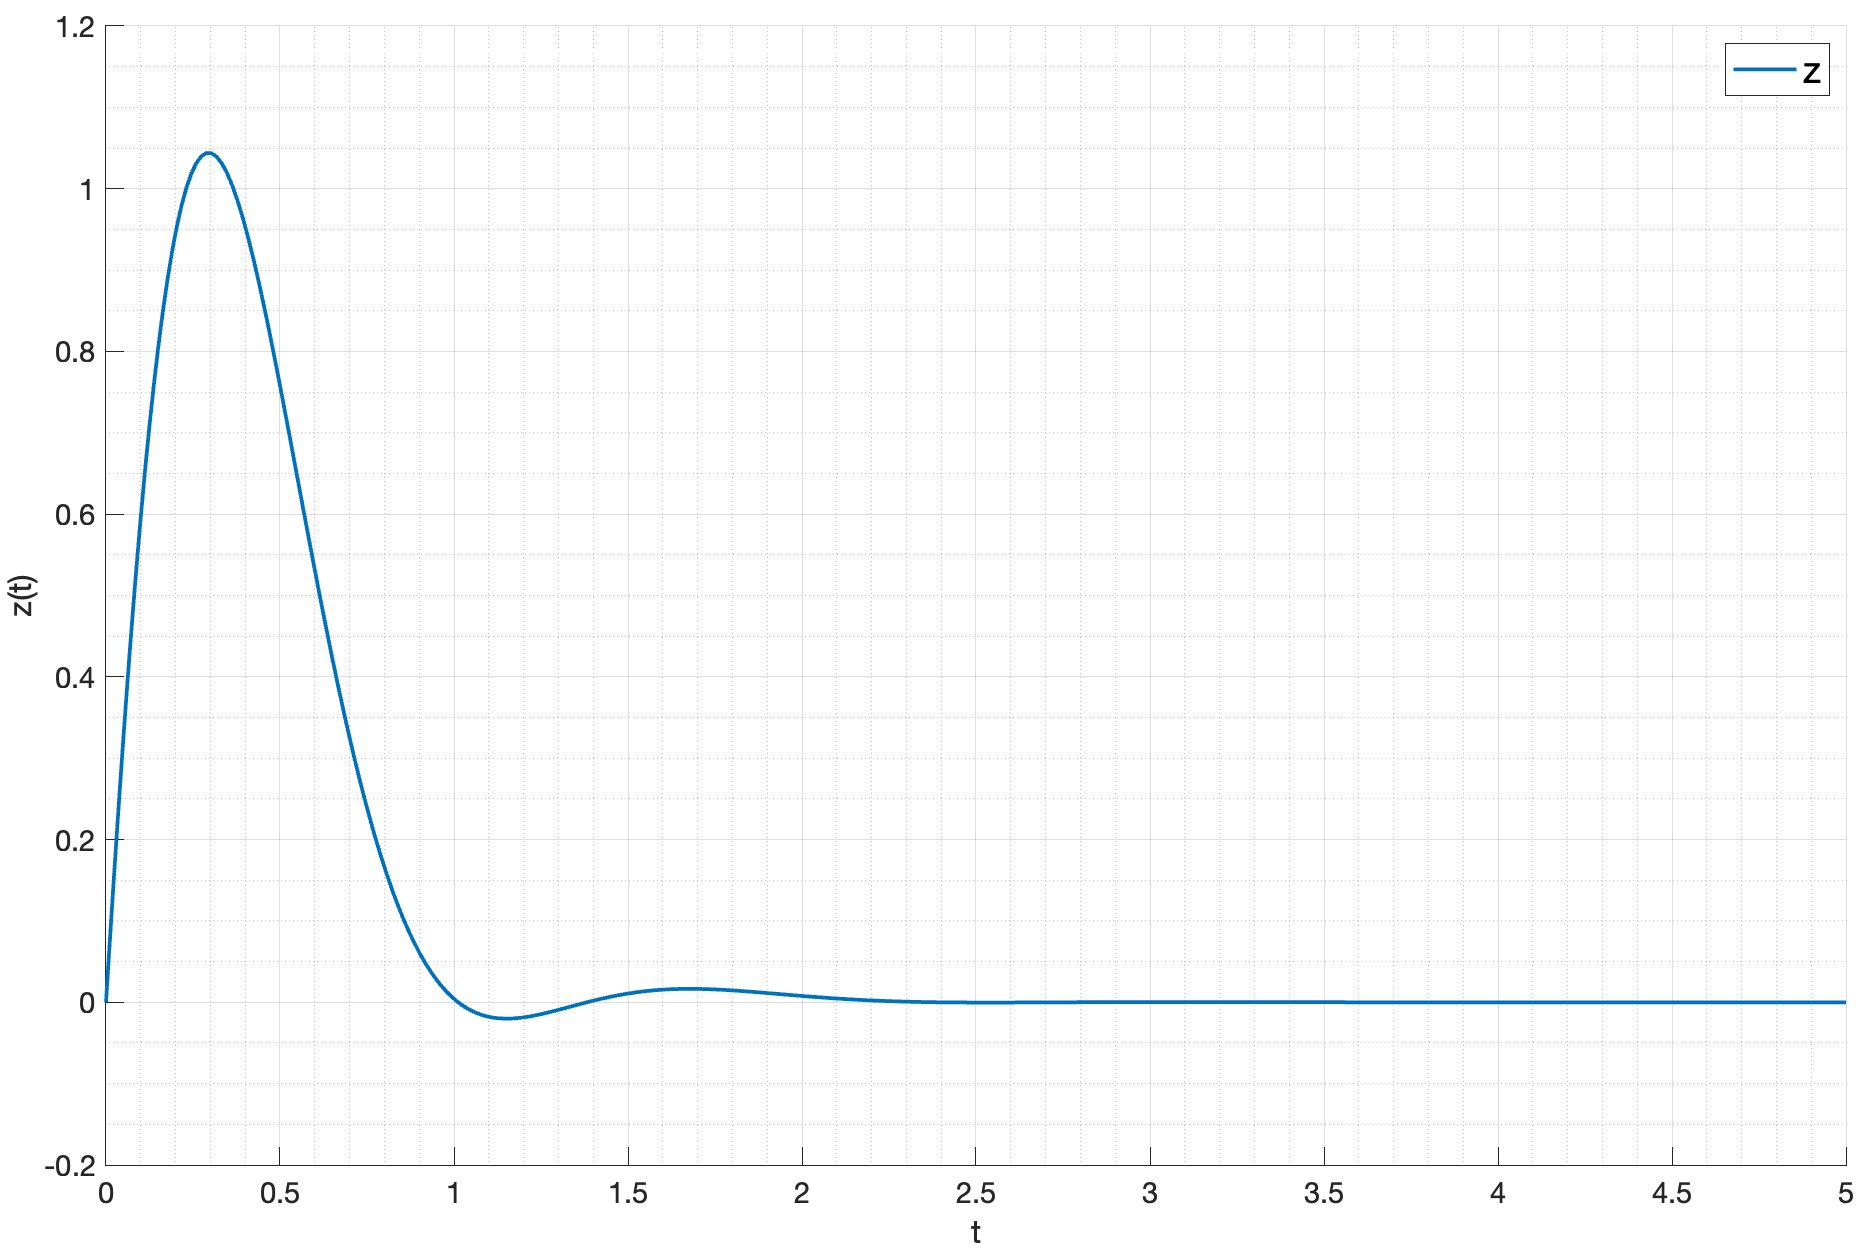
\includegraphics[width=\textwidth]{media/plots/full_z.png}
    \caption{Выход системы с полным регулятором $K_1 + K_2$}
    \label{fig:K_full_z}
\end{figure}
График управления, полученного с помощью полных регуляторов $K_1 + K_2$ приведен на рисунке \ref{fig:K_full_u}.
\begin{figure}[ht!]
    \centering
    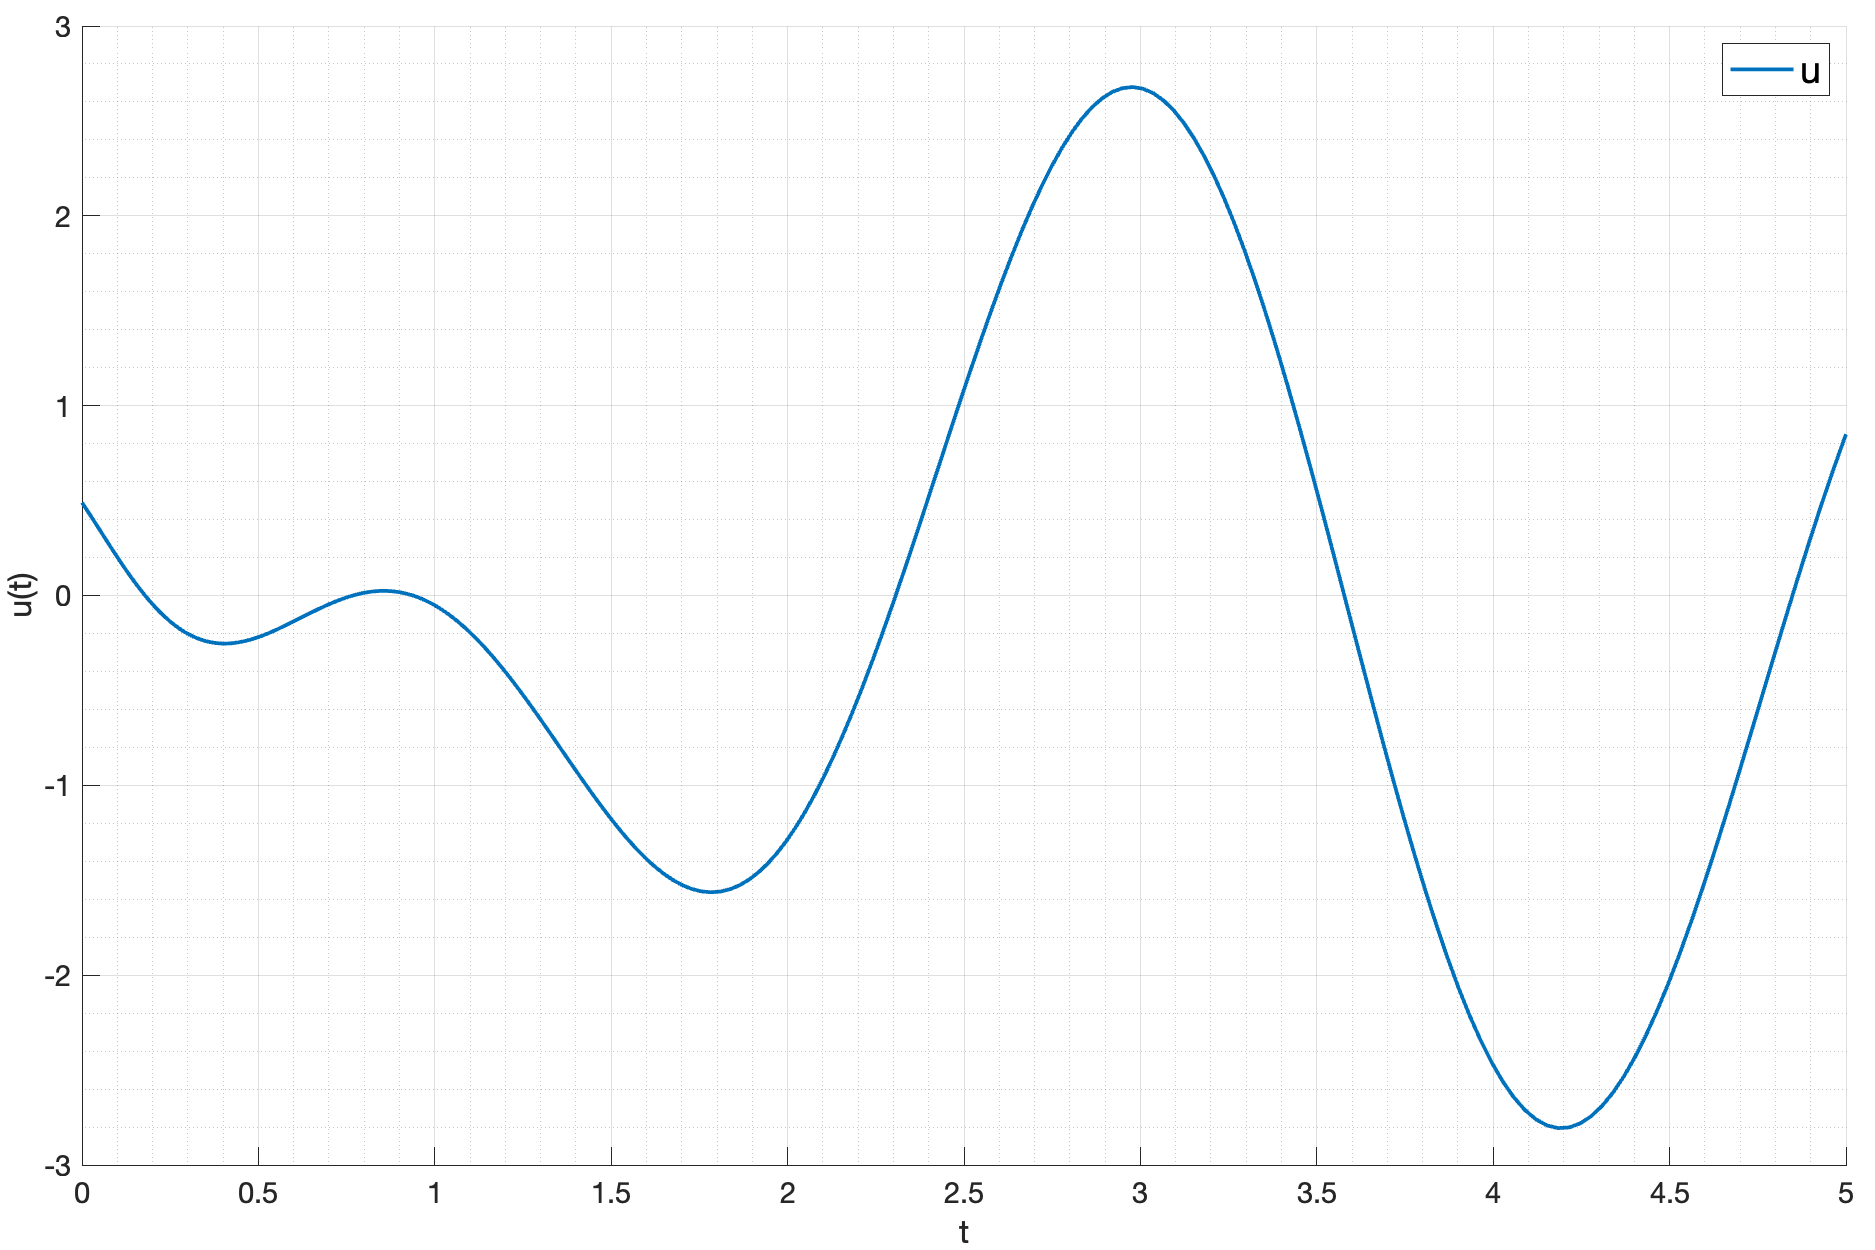
\includegraphics[width=\textwidth]{media/plots/full_u.png}
    \caption{Управление системы с полным регулятором $K_1 + K_2$}
    \label{fig:K_full_u}
\end{figure}
Видно, что выход системы сходится к нулю, что подтверждает корректность синтеза регулятора. 
\FloatBarrier

Сравнительные графики управления, формируемого разными регуляторами приведены на рисунке \ref{fig:compare_u}.
\begin{figure}[ht!]
    \centering
    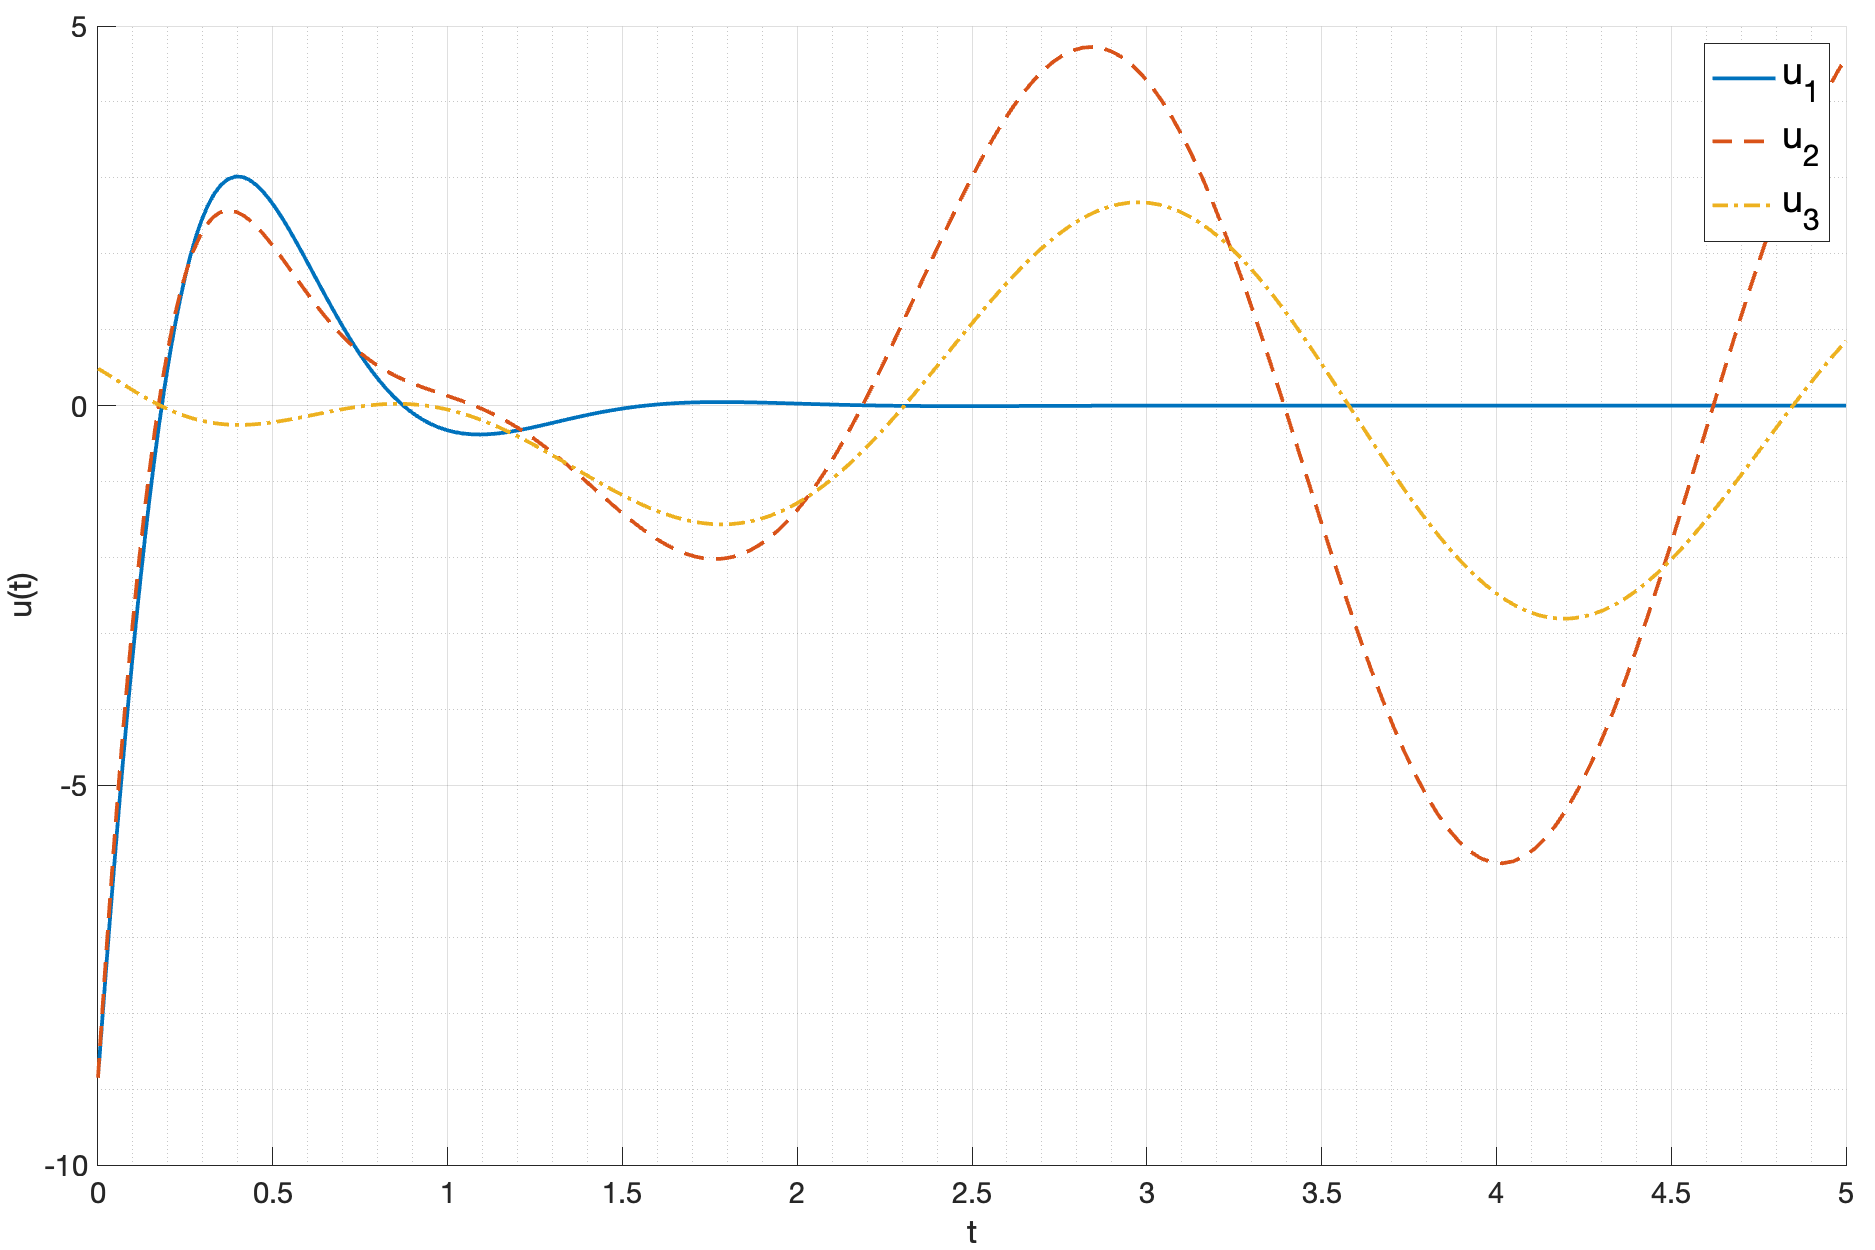
\includegraphics[width=\textwidth]{media/plots/u_cmp.png}
    \caption{Сравнение управления, формируемого разными регуляторами}
    \label{fig:compare_u}
\end{figure}
где $u_1$ -- управление, формируемое регулятором $K_1$ без внешнего воздействия, $u_2$ -- управление, формируемое полным регулятором $K_1$ 
с внешним воздействием, $u_3$ -- управление, формируемое полным регулятором $K_1 + K_2$ с внешним воздействием.

Сравнительные графики виртуального выхода, формируемого разными регуляторами приведены на рисунке \ref{fig:compare_z}.
\begin{figure}[ht!]
    \centering
    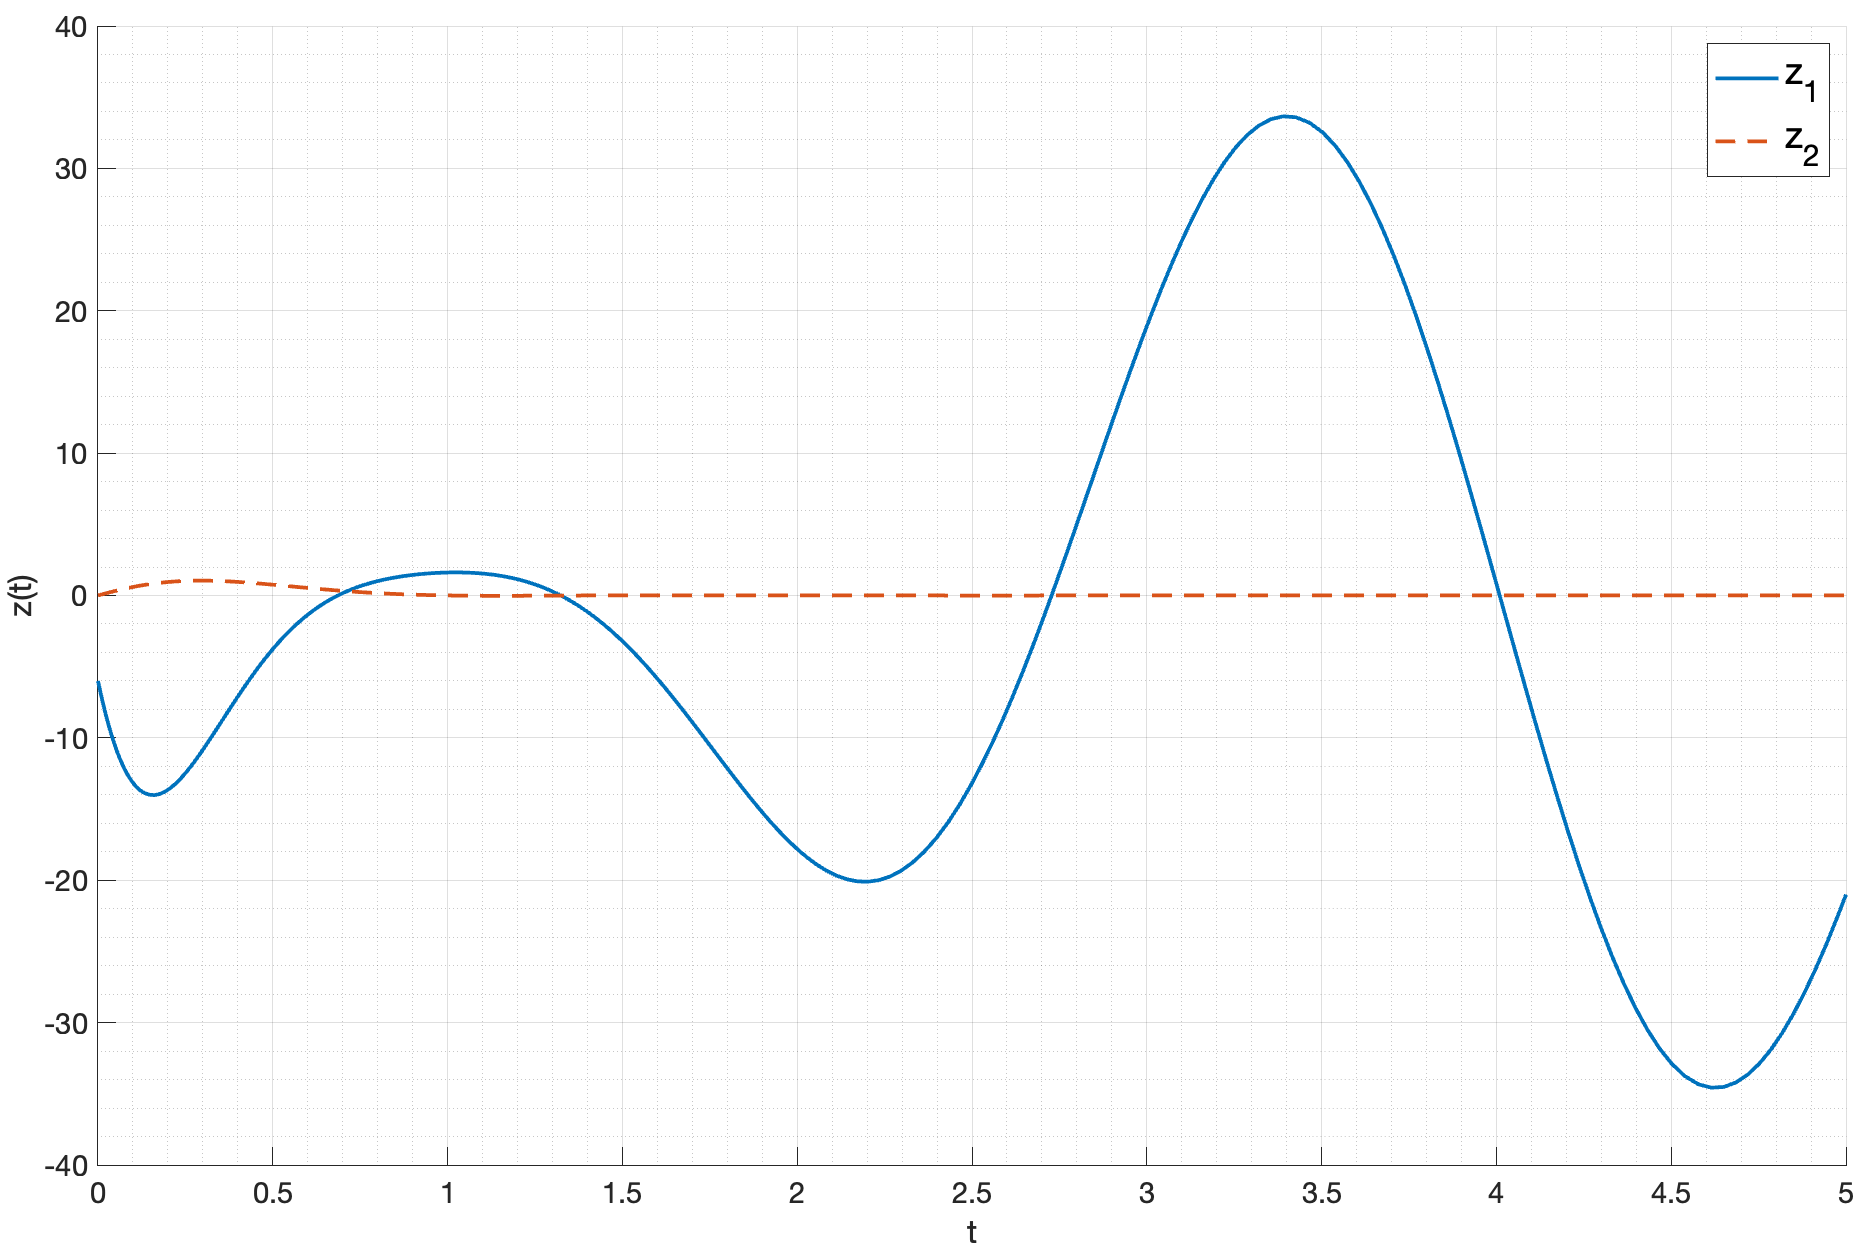
\includegraphics[width=\textwidth]{media/plots/z_cmp.png}
    \caption{Сравнение виртуального выхода, формируемого разными регуляторами}
    \label{fig:compare_z}
\end{figure}
где $z_1$ -- выход системы с регулятором $K_1$ с внешним воздействием, $z_2$ -- выход системы с полным регулятором $K_1 + K_2$ с внешним воздействием.
\FloatBarrier

\subsection{Выводы}
В результате исследования системы с внешним возмущением и различными регуляторами
можно сделать следующие выводы: система с \textit{классическим} немодальным регулятором
$K_1$ не является устойчивой при наличии внешнего возмущения, содержащего гармонические
составляющие. Система с \textit{полным} регулятором $K_1 + K_2$ является устойчивой при наличии 
внешнего возмущения. При этом состояние системы с полным регулятором не сходится к нулю,
компенсируя внешнее возмущение. 